\documentclass[11pt,a4paper]{article}
\usepackage[utf8]{inputenc}
\usepackage[T1]{fontenc}
\usepackage[spanish,es-noshorthands]{babel}
\usepackage{lmodern}
\usepackage[margin=2.5cm]{geometry}
\usepackage{booktabs}
\usepackage{tabularx}
\usepackage{enumitem}
\usepackage{graphicx}
\usepackage{float}
\usepackage{listings}
\usepackage{amsmath}
\usepackage{tikz}
\usetikzlibrary{positioning,arrows.meta,fit,shapes.misc}
\usepackage[hidelinks]{hyperref}

\newcolumntype{Y}{>{\raggedright\arraybackslash}X}
\newcommand{\code}[1]{\texttt{#1}}
\graphicspath{{figuras/}}

\lstset{
  basicstyle=\ttfamily\small,
  frame=single,
  columns=fullflexible,
  keepspaces=true,
  breaklines=true,
  showstringspaces=false,
  xleftmargin=4pt,
  xrightmargin=4pt,
}

\title{Motor de base de datos multimodal en disco\\
\large Base de Datos II (CS2042) --- Proyecto 2: módulos espacial, textual,
vectorial y aplicación de IA}
\author{Sebastian Hernandez Miñano \and David Huette Ospino \and
Luis Millones Carrasco \and Isaac Gamero del Aguila}
\date{Noviembre de 2026}

\begin{document}
\maketitle

\begin{center}
Repositorio: \url{https://github.com/Davidht77/proyecto-1-bd2}
\end{center}

% Cada sección vive en su propio archivo para que cada rol edite el suyo sin
% conflictos. El documento maestro solo fija el preámbulo y el orden.
%
%   secciones/introduccion.tex   arquitectura multimodal y reglas comunes  (Rol 4)
%   secciones/espacial.tex       R-Tree + Experimento 5                     (Rol 1)
%   secciones/textual.tex        índice invertido + Experimento 6           (Rol 2)
%   secciones/vectorial.tex      IVF + planificador híbrido + Experimento 8 (Rol 3)
%   secciones/multimedia.tex     BoVW vs embeddings, RAG + Experimento 7    (Rol 4)
%   secciones/conclusiones.tex

\section{Resumen y arquitectura multimodal}

El Entregable 1 dejó un motor relacional que guarda todo en páginas binarias de
tamaño fijo y cuenta cada transferencia con un \code{DiskCounter}. El Entregable 2 lo
extiende para indexar y recuperar tres clases de datos no convencionales
---geometrías, texto libre y vectores de alta dimensión--- y lo usa como base de una
aplicación de inteligencia artificial completa. Cuatro reglas atraviesan todos los
módulos nuevos:

\begin{enumerate}[nosep]
  \item \textbf{Solo el \code{Pager} toca el disco.} Cada índice nuevo (R-Tree,
        vocabulario B+, postings, directorio y listas del IVF, archivo de normas) es un
        archivo paginado con la misma cabecera de 32 bytes del Proyecto 1. Por eso el
        desglose de bloques leídos por consulta sigue siendo exacto y comparable entre
        módulos.
  \item \textbf{Archivos autodescriptivos.} La página 0 de cada archivo guarda su
        esquema; el catálogo reconstruye tablas e índices escaneando el directorio, sin
        metadatos externos ni serializadores de alto nivel.
  \item \textbf{Una sola gramática.} El parser SQL del Proyecto 1 se extendió con
        \code{POINT}, \code{VECTOR(D)}, \code{USING RTREE | INVERTED | IVF},
        \code{WITHIN\_RADIUS}, \code{KNN}, \code{MATCH}, los operadores \code{<->} /
        \code{<=>} y \code{SET}. El planificador decide la ruta de acceso y la
        reporta junto al I/O de índice y de tabla.
  \item \textbf{Todo lo persistente de la aplicación de IA son tablas e índices del
        motor.} El corpus del RAG, los embeddings, el codebook de palabras visuales y
        las imágenes indexadas viven en tablas \code{HEAP} con columnas
        \code{VECTOR(D)} y en los índices anteriores, no en estructuras paralelas.
\end{enumerate}

\subsection{Mapa de componentes}

\begin{figure}[H]
\centering
\begin{tikzpicture}[
  node distance=4mm and 6mm,
  caja/.style={draw, rounded corners=1pt, align=center, font=\small, inner sep=4pt, minimum height=8mm},
  capa/.style={draw, dashed, rounded corners=2pt, inner sep=5pt},
  flecha/.style={-{Latex[length=2mm]}, thick},
]
\node[caja, fill=blue!6] (web) {Cliente web (React)\\ SQL · mapa Leaflet · RAG · multimedia};
\node[caja, fill=blue!6, below=of web] (api) {API REST (FastAPI)\\ \code{/api/query} · \code{/api/rag/*} · \code{/api/multimedia/*}};
\node[caja, below=of api] (exec) {Parser SQL multimodal + planificador híbrido\\ \code{SeqScan} · \code{IndexScan} · \code{SpatialSeqScan}/R-Tree · \code{KnnSeqScan} · \code{IVFScan} · \code{PreFilter}/\code{PostFilter}};
\node[caja, below left=6mm and -22mm of exec, fill=green!6] (rt) {R-Tree\\ \code{.rtree.dat}};
\node[caja, right=of rt, fill=green!6] (inv) {Índice invertido\\ \code{vocab} B+ · \code{postings} · \code{norms}};
\node[caja, right=of inv, fill=green!6] (ivf) {IVF\\ \code{.ivf.dir} · \code{.ivf.lst}};
\node[caja, right=of ivf, fill=green!6] (rel) {B+ · Hash\\ (Proyecto 1)};
\node[caja, below=8mm of inv, xshift=14mm, fill=orange!8] (pager) {\code{Pager} + \code{DiskCounter} + \code{Page} (bloques de 4 KB, RID $\langle$page, slot$\rangle$)};
\node[caja, below=of pager] (disk) {Heap File · Sequential File · archivos de índice};
\node[caja, left=10mm of rt, fill=red!5, text width=30mm] (ia) {Modelos de IA\\ SIFT+K-Means · ResNet-18\\ SBERT · LLM};
\draw[flecha] (web) -- (api);
\draw[flecha] (api) -- (exec);
\foreach \n in {rt,inv,ivf,rel} \draw[flecha] (exec) -- (\n);
\foreach \n in {rt,inv,ivf,rel} \draw[flecha] (\n) -- (pager);
\draw[flecha] (pager) -- (disk);
\draw[flecha, dashed] (ia) |- (api);
\end{tikzpicture}
\caption{Arquitectura del Entregable 2. Los modelos de IA solo producen vectores o
texto; todo lo que se persiste y se consulta pasa por el motor y su contador de I/O.}
\end{figure}

\subsection{Reparto del trabajo}

\begin{table}[H]
\centering\small
\begin{tabularx}{\textwidth}{lY}
\toprule
Rol & Entregables \\
\midrule
1 --- Espacial & R-Tree en disco (MBR, split cuadrático, rango y k-NN), visor Leaflet, Experimento 5. \\
2 --- Texto & Preprocesamiento (Snowball es/en), SPIMI, vocabulario B+ + postings, booleano, BM25 / TF-IDF, Experimento 6. \\
3 --- Vectorial y SQL & \code{VECTOR(D)}, k-NN exacto con Max-Heap, IVF en disco, gramática multimodal, planificador PRE/POST con I/O desglosado, Experimento 8. \\
4 --- Multimedia e IA & BoVW (SIFT + K-Means + índice invertido con TF-IDF coseno) vs. embeddings densos (ResNet-18, SBERT) + IVF; aplicación RAG sobre Wikipedia con cliente LLM multiproveedor; Experimento 7; README, informe y video. \\
\bottomrule
\end{tabularx}
\end{table}

\subsection{Condiciones de medición}

Todos los experimentos corren con bloques de 4096 bytes y sin buffer pool
(\code{BD2\_CACHE\_SIZE=0}), de modo que cada lectura de página es una transferencia
real y el número de bloques es independiente de la máquina. Las latencias se midieron
en un portátil con CPU Intel i7-13620H sin GPU, 16 GB de RAM y disco SSD, bajo
Windows 11 y Python 3.12; por eso el análisis prioriza los bloques leídos y usa la
latencia como confirmación.

\section{Módulo espacial: R-Tree en disco}
\label{sec:espacial}

% Cuerpo tomado de experimento5_rtree.tex (Rol 1) por un script; si editas
% el original, vuelve a correr: python informe_analisis/secciones/sincronizar_espacial.py


\subsection{Objetivo y alcance}

El módulo espacial agrega un índice \textbf{R-Tree} para columnas geográficas y dos
predicados SQL: \code{WITHIN\_RADIUS} y \code{KNN}. El índice se persiste en disco
sobre las mismas páginas de tamaño fijo que usan el Heap File y los demás índices;
ninguna estructura se mantiene solo en memoria. Todas las lecturas y escrituras
pasan por el \code{Pager}, de modo que el \code{DiskCounter} sigue siendo la fuente
única de la telemetría.

El alcance incluye:

\begin{itemize}
  \item tipo de columna \code{POINT} (par \code{(lon, lat)} en \code{float64});
  \item \code{CREATE INDEX ... USING RTREE};
  \item \code{<col> WITHIN\_RADIUS ((x, y), r)} con refinamiento haversine;
  \item \code{<col> KNN ((x, y), k)} con cola de prioridad por \code{MINDIST};
  \item plan de respaldo sin índice (\emph{spatial sequential scan});
  \item visor de mapa en el cliente web y el Experimento 5.
\end{itemize}

\subsection{Estructura en disco}

\subsubsection{Páginas y entradas}

El R-Tree usa dos tipos de página nuevos, \code{RT\_INTERNAL = 6} y
\code{RT\_LEAF = 7}, con la cabecera habitual de 32 bytes. El archivo se llama
\code{<tabla>\_\_<índice>.rtree.dat} y guarda en la cabecera del \code{Pager}:

\begin{itemize}
  \item \code{user\_a}: \code{root\_page\_id};
  \item \code{user\_b}: altura del árbol (con la raíz en el nivel 1).
\end{itemize}

Cada entrada mide \code{8D + 10} bytes:

\begin{center}
\begin{tabular}{lll}
\hline
Campo & Tipo & Bytes \\
\hline
MBR & \code{2D} coordenadas \code{float32} & \(8D\) \\
RID & \code{page\_id}, \code{slot}, \code{area}, \code{flags} & 10 \\
\hline
\end{tabular}
\end{center}

En 2D la entrada mide 26 bytes. Con páginas de 4096 bytes el fan-out es de 155
entradas por nodo: la capacidad se resuelve con la fórmula del bitmap de slots,
\(\lfloor 8(B-H)/(8R+1) \rfloor\). Un nodo interno almacena
\code{<MBR, página hija>}; una hoja almacena \code{<MBR, RID>}, donde el MBR de
un punto es el punto repetido en las dos esquinas.

El RID es \emph{físico}: identifica la página, el slot y si la fila vive en el
área principal o en la cadena de overflow. Esto permite resolver la fila con una
sola lectura, sin volver a buscar por clave primaria.

\subsubsection{Esquema autodescriptivo}

Para reutilizar el \code{Pager} y el formato de archivo del resto del sistema,
el R-Tree escribe una cabecera con un \code{Schema} ficticio de dos columnas:
la primera describe el MBR como \code{POINT} y la segunda absorbe los bytes
restantes como \code{CHAR}. La dimensión se recupera del tamaño de registro:
\(D = (\text{record\_size} - 8) / 8\). Así el catálogo puede abrir el índice sin
un archivo de metadatos adicional.

\subsection{Algoritmos}

\subsubsection{Inserción}

La inserción desciende desde la raíz eligiendo en cada nodo interno el hijo cuyo
MBR crece menos al incluir el punto; el desempate usa el área actual del MBR.
Al llegar a una hoja se agrega la entrada y, si se supera la capacidad, se
divide el nodo. La división es la \textbf{cuadrática} clásica de Guttman:

\begin{enumerate}
  \item se eligen como semillas el par de entradas cuya unión desperdicia más
        área (\(\text{área}(A \cup B) - \text{área}(A) - \text{área}(B)\));
  \item cada entrada restante se asigna al grupo cuya área crece menos, con
        desempate por balance de ocupación.
\end{enumerate}

Si la raíz se divide, se crea una nueva raíz interna con dos hijos y la altura
aumenta en uno. La carga masiva usa \textbf{STR} (\emph{Sort-Tile-Recursive}):
ordena por la primera coordenada, parte en franjas, ordena cada franja por la
segunda coordenada y llena las hojas en orden. El resultado es un árbol
balanceado y con alta ocupación sin pagar una inserción por fila.

\subsubsection{Búsqueda por ventana}

\code{WITHIN\_RADIUS} se traduce a la caja conservadora que contiene el círculo
(ajustando la longitud por \(\cos(\text{lat})\)) y recorre el árbol podando toda
rama cuyo MBR no intersecta la ventana. Las entradas de las hojas que sí
intersectan se convierten a RID y se leen de la tabla. Como la caja incluye las
esquinas del círculo, el resultado se refina con la distancia haversine exacta;
así no se devuelven falsos positivos.

\subsubsection{k-NN}

\code{KNN} usa búsqueda \emph{best-first}. Una cola de prioridad guarda nodos
ordenados por \code{MINDIST(Q, MBR)}, la distancia mínima del centro de consulta
al rectángulo. Se extrae el nodo más prometedor; si su cota inferior ya supera la
distancia del \(k\)-ésimo vecino encontrado, se poda el resto. En las hojas se
calcula la distancia exacta con haversine (o euclídea si el índice no es
geográfico). El resultado sale ordenado de menor a mayor distancia.

\subsection{Integración con el motor SQL}

El parser reconoce \code{POINT} como tipo de columna y como literal
(\code{POINT(x, y)}), y agrega los nodos \code{SpatialRadius} y \code{SpatialKNN}.
El ejecutor elige el plan:

\begin{center}
\begin{tabular}{lll}
\hline
Predicado & Con índice & Sin índice \\
\hline
\code{WITHIN\_RADIUS} & \code{RTreeRangeScan} & \code{SpatialSeqScan} \\
\code{KNN} & \code{RTreeKNN} & \code{SpatialSeqScan} + orden \\
\hline
\end{tabular}
\end{center}

El plan incluye el nombre del índice, la columna, el radio o \(k\), y los MBR
visitados. La respuesta JSON agrega un bloque \code{spatial} con el centro, el
tipo de consulta y \code{visited\_mbrs}; el cliente web lo usa para dibujar el
recorrido del árbol.

\begin{verbatim}
CREATE TABLE locales (
  id INT PRIMARY KEY,
  nombre CHAR(20),
  ubicacion POINT
) USING HEAP;

INSERT INTO locales VALUES (1, 'Miraflores', POINT(-77.0282, -12.1354));

CREATE INDEX idx_geo ON locales (ubicacion) USING RTREE;

SELECT id, nombre FROM locales
WHERE ubicacion WITHIN_RADIUS ((-77.0282, -12.1354), 2.5);

SELECT id, nombre FROM locales
WHERE ubicacion KNN ((-77.0282, -12.1354), 10);
\end{verbatim}

\paragraph{Mantenimiento.} En un Heap File un \code{INSERT} agrega la entrada al
R-Tree con el RID recién asignado: la fila nueva no mueve a las anteriores. En
un Sequential File, en cambio, la inserción ordenada desplaza slots dentro de la
página y los splits de overflow mueven registros entre páginas; cualquiera de
esos eventos invalida RIDs ajenos. Por eso el ejecutor reconstruye el R-Tree
después de cada inserción en una tabla Sequential. Es correcto, pero conviene
crear el índice después de la carga masiva (o usar Heap) para no pagar un
reindexado por fila. Un \code{DELETE} también reconstruye el índice: el Heap
borra con \emph{move-the-last} y el Sequential File puede mover filas al
reorganizar. La reorganización explícita del Sequential File dispara la misma
reconstrucción.

\subsection{Cliente web}

La pestaña \textbf{Mapa espacial} aparece cuando la consulta devuelve un bloque
\code{spatial}. Usa Leaflet para dibujar:

\begin{itemize}
  \item los puntos devueltos, con un marcador por fila;
  \item el centro de la consulta y el círculo del radio (o el centro del k-NN);
  \item los MBR de los nodos visitados como rectángulos punteados.
\end{itemize}

El mapa se encuadra automáticamente sobre los puntos y el área de búsqueda.

\subsection{Metodología del Experimento 5}

Los datos son puntos aleatorios uniformes en una caja alrededor de Lima
(\(-77{,}35\) a \(-76{,}70\) de longitud y \(-12{,}43\) a \(-11{,}84\) de latitud).
Se comparan dos alternativas sobre el mismo conjunto:

\begin{itemize}
  \item \textbf{R-Tree}: se mide solo la lectura de páginas del índice durante la
        consulta; la resolución de los RID y el filtro haversine se hacen en
        memoria.
  \item \textbf{Secuencial}: se recorre el Heap File completo, se calcula la
        distancia de cada fila y se filtran u ordenan los resultados.
\end{itemize}

Para cada \(N \in \{10\,000, 50\,000, 100\,000\}\) se lanzan 30 consultas con
centros elegidos al azar entre los mismos puntos. La suite de radio usa
selectividades de \(0{,}1\%\), \(1\%\), \(5\%\), \(10\%\) y \(25\%\); la suite
k-NN usa \(k \in \{5, 20, 50\}\). La suite dimensional construye R-Trees de
\(D = 2, 4, 8, 16, 32, 64, 128\) con \(N = 10\,000\) y consulta una ventana que
cubre el \(1\%\) del volumen; el costo secuencial es la fórmula analítica
\(\lceil N / \text{capacidad}(4096, 8D+4) \rceil\). Todas las corridas usan
páginas de 4096 bytes y buffer pool apagado.

\subsection{Resultados}

\subsubsection{Consultas por radio}

\begin{figure}[htbp]
  \centering
  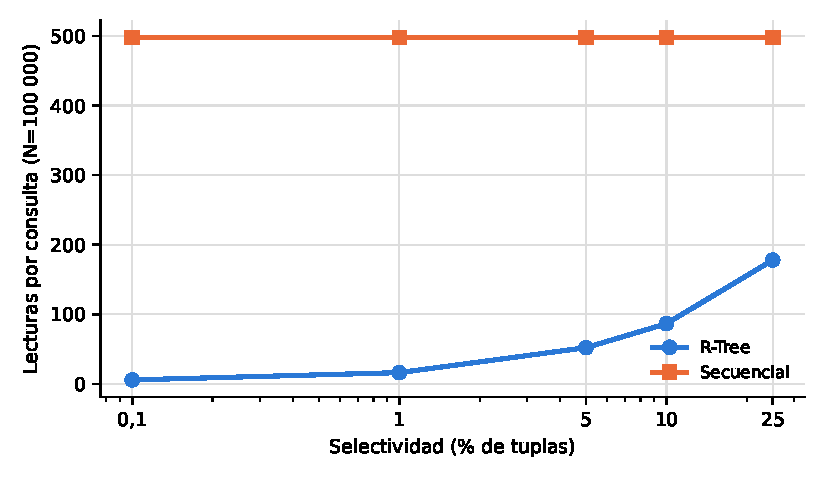
\includegraphics[width=0.75\textwidth]{exp5_radio.pdf}
  \caption{Lecturas por consulta para \code{WITHIN\_RADIUS} con \(N = 100\,000\).}
\end{figure}

\begin{center}
\begin{tabular}{rrrr}
\hline
 & \multicolumn{3}{c}{Lecturas por consulta} \\
\cline{2-4}
Selectividad & R-Tree (\(N=10^4\)) & R-Tree (\(N=10^5\)) & Secuencial (\(N=10^5\)) \\
\hline
0,1\,\% & 2,7 & 5,7 & 498 \\
1\,\%   & 4,5 & 16,3 & 498 \\
5\,\%   & 8,7 & 52,1 & 498 \\
10\,\%  & 13,6 & 86,6 & 498 \\
25\,\%  & 23,1 & 178,0 & 498 \\
\hline
\end{tabular}
\end{center}

\begin{itemize}
  \item El escaneo secuencial siempre lee las 498 páginas del Heap, sin importar
        la selectividad: su costo es \(P\).
  \item Con \(N = 100\,000\) y \(0{,}1\%\) de selectividad, el R-Tree lee 5,7
        páginas, unas 87 veces menos. Incluso con \(25\%\) de selectividad lee
        178, todavía por debajo del full scan.
  \item Al crecer \(N\), el R-Tree agrega niveles pero el costo crece mucho más
        despacio que \(P\): entre \(N=10^4\) y \(N=10^5\) las lecturas se
        duplican, mientras que el escaneo se multiplica por 10.
  \item La latencia sigue el mismo orden: para \(N=100\,000\) el R-Tree tarda
        entre 3 y 159 ms según la selectividad, frente a \(\approx 197\) ms del
        escaneo completo.
\end{itemize}

\subsubsection{k vecinos más cercanos}

\begin{figure}[htbp]
  \centering
  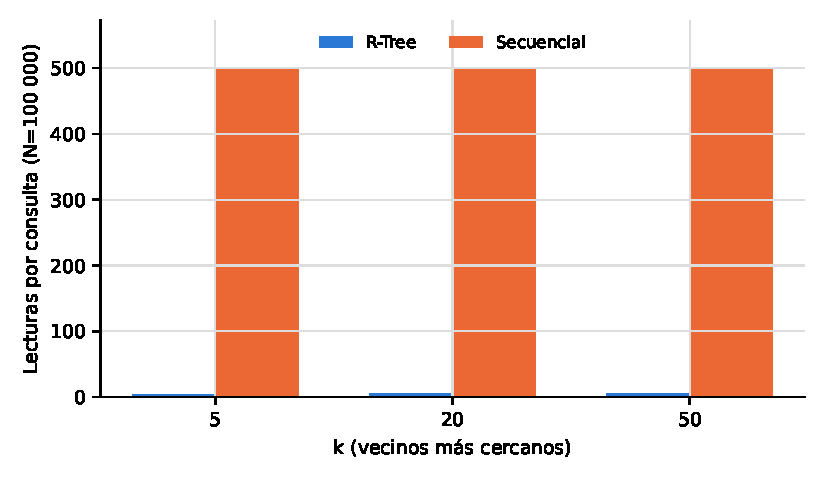
\includegraphics[width=0.75\textwidth]{exp5_knn.pdf}
  \caption{Lecturas por consulta para \code{KNN} con \(N = 100\,000\).}
\end{figure}

\begin{center}
\begin{tabular}{rrrr}
\hline
 & \multicolumn{3}{c}{Lecturas por consulta} \\
\cline{2-4}
\(k\) & R-Tree (\(N=10^4\)) & R-Tree (\(N=10^5\)) & Secuencial (\(N=10^5\)) \\
\hline
5  & 3,5 & 4,6 & 498 \\
20 & 4,0 & 5,0 & 498 \\
50 & 4,6 & 5,6 & 498 \\
\hline
\end{tabular}
\end{center}

El costo del R-Tree es casi constante: la cola de prioridad baja por una rama y
poda el resto en cuanto la cota inferior supera al \(k\)-ésimo vecino. Pasar de
\(k=5\) a \(k=50\) agrega apenas una página. El escaneo, en cambio, no puede
evitar leer la tabla completa y además ordena \(N\) distancias: con
\(N=100\,000\) tarda \(\approx 279\) ms por consulta, frente a \(\approx 1\) ms
del R-Tree. La diferencia en lecturas es de 498 a 4,6 páginas.

\subsubsection{Maldición de la dimensionalidad}

\begin{figure}[htbp]
  \centering
  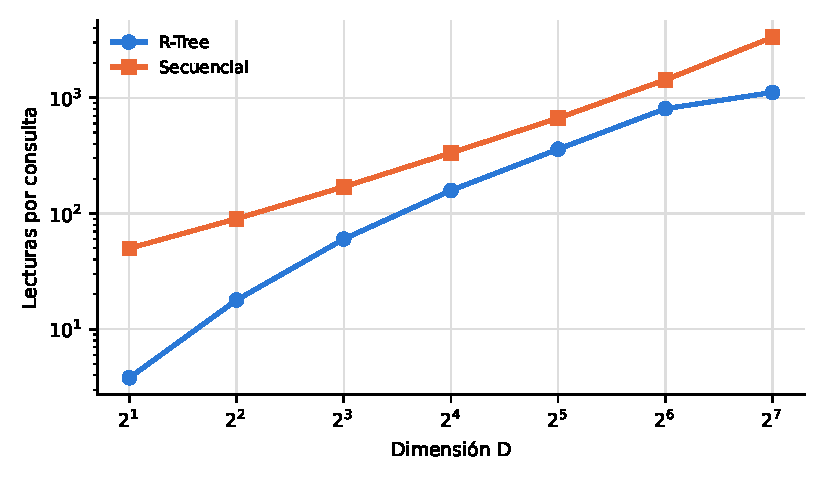
\includegraphics[width=0.75\textwidth]{exp5_dimension.pdf}
  \caption{Lecturas por consulta según la dimensión del R-Tree (\(N = 10\,000\)).}
\end{figure}

\begin{center}
\begin{tabular}{rrrr}
\hline
\(D\) & Lecturas R-Tree & Lecturas full scan & Filas devueltas \\
\hline
2   & 3,8    & 50    & 96,2 \\
4   & 17,9   & 90    & 76,5 \\
8   & 60,1   & 170   & 26,3 \\
16  & 158,3  & 334   & 4,0 \\
32  & 359,6  & 667   & 1,0 \\
64  & 804,6  & 1\,429 & 1,0 \\
128 & 1\,112,5 & 3\,334 & 1,0 \\
\hline
\end{tabular}
\end{center}

\begin{itemize}
  \item Hasta \(D=4\) el R-Tree lee entre 4 y 5 veces menos que el full scan.
  \item A partir de \(D=8\) los MBR se solapan casi por completo: la poda deja
        de ser selectiva y el árbol termina visitando una fracción grande de las
        hojas.
  \item Con \(D=128\) el R-Tree todavía lee menos que el escaneo, pero la ventaja
        se reduce a un factor de 3 y el árbol ocupa muchos más niveles. Es el
        comportamiento esperado: los índices multidimensionales dejan de ser
        útiles cuando la dimensión se acerca al número de filas por página.
\end{itemize}

\subsection{Conclusiones}

\begin{itemize}
  \item El R-Tree reduce el costo de \code{WITHIN\_RADIUS} de \(O(P)\) a
        \(O(\text{hojas visitadas})\), con una ventaja de hasta dos órdenes de
        magnitud en consultas selectivas.
  \item \code{KNN} mantiene un costo casi constante respecto de \(k\), porque la
        cota \code{MINDIST} poda las ramas que no pueden mejorar al vecino actual.
  \item La poda por MBR funciona bien en 2D y se degrada con la dimensión: el
        experimento reproduce la maldición de la dimensionalidad.
  \item Persistir el árbol en páginas de tamaño fijo y reutilizar el
        \code{Pager} mantiene el conteo de I/O exacto y permite comparar el
        índice con el escaneo secuencial en igualdad de condiciones.
  \item La reconstrucción tras \code{DELETE} y reorganización es el precio de
        usar RID físicos; a cambio, resolver una fila cuesta una sola lectura.
\end{itemize}


\section{Módulo textual: índice invertido en disco}
\label{sec:textual}

\subsection{Pipeline léxico y SPIMI}

El preprocesamiento (\code{backend/text/preprocess.py}) tokeniza con una expresión
regular de letras Unicode, pasa a minúsculas, elimina las stopwords de NLTK en
español e inglés y aplica el stemmer Snowball del idioma detectado (el que más
stopwords aporta al documento; la consulta pasa por los dos stemmers). Cada término
se corta a 24 bytes porque el vocabulario lo guarda en un \code{CHAR} de ancho fijo.

La construcción es SPIMI (\code{spimi.py}): una pasada sobre los documentos acumula
término $\to$ postings en RAM hasta un presupuesto de postings, vuelca cada bloque
ordenado a disco y al final hace un merge de $k$ vías con un heap, leyendo una
página por bloque. Como el merge es estable y la tabla se recorre en orden de RID,
cada lista de posteo queda ordenada por RID sin reordenarla.

\subsection{Diseño en disco}

Un índice \code{INVERTED} sobre la columna de una tabla son cuatro archivos paginados
por el \code{Pager}:

\begin{table}[H]
\centering\small
\begin{tabularx}{\textwidth}{lY}
\toprule
Archivo & Contenido \\
\midrule
\code{<t>\_\_<idx>.inv.meta} & cabecera autodescriptiva: la columna indexada, el ranking por defecto (\code{user\_a}) y si el índice quedó desactualizado (\code{user\_b}) \\
\code{...inv.vocab.dic} & diccionario: un árbol B+ del Proyecto~1 con clave \code{CHAR(24)} (el término $t$) y valor $\langle$offset de la lista en \code{postings.inv}, $df_t\rangle$; como cada documento aparece una vez por término, el largo de la lista de posteo es $df_t$ \\
\code{...inv.postings.inv} & listas de posteo: un arreglo contiguo de registros $\langle$page, slot, $tf_{t,d}$, $|d|\rangle$ de 16 bytes (252 por página), con las listas una detrás de otra y ordenadas por RID; $N$ y $\sum|d|$ van en la cabecera \\
\code{...inv.norms.dat} & la norma euclidiana $\|\vec d\|_2$ de cada documento, precalculada para el coseno \\
\bottomrule
\end{tabularx}
\caption{Archivos del índice invertido.}
\end{table}

\begin{figure}[H]
\centering
\begin{tikzpicture}[
  pg/.style={draw, rounded corners=1pt, minimum width=1.5cm, minimum height=0.85cm,
             font=\scriptsize, align=center},
  >={Stealth[length=2mm]}, node distance=0.22cm]
  \node[font=\footnotesize\bfseries, anchor=west] at (-0.8,3.1) {\texttt{vocab.dic} (B+): término $\to$ (offset, $df$)};
  \node[pg, fill=blue!10] (r) at (3.2,2.35) {raíz};
  \node[pg, fill=blue!6] (h1) at (0.6,1.4) {hoja\\\texttt{guerr}: (812, 37)};
  \node[pg, fill=blue!6, right=of h1] (h2) {hoja\\\texttt{histori}: (849, 61)};
  \node[right=of h2] (hd) {$\cdots$};
  \draw[->] (r) -- (h1.north);
  \draw[->] (r) -- (h2.north);
  \draw[->, dashed] (h1) -- (h2);

  \node[font=\footnotesize\bfseries, anchor=west] at (-0.8,-1.2) {\texttt{postings.inv}: un arreglo contiguo, listas ordenadas por RID};
  \node[pg, fill=gray!15] (p0) at (0,-0.4) {pág.\ 0\\$N$, $\sum|d|$};
  \node[pg, fill=orange!18, right=of p0] (p1) {pág.\ 1};
  \node[right=of p1] (pd) {$\cdots$};
  \node[pg, fill=orange!18, right=of pd] (p4) {pág.\ 4\\pos.\ 812..};
  \node[pg, fill=orange!18, right=of p4] (p5) {pág.\ 4--5\\pos.\ 849..};
  \draw[->, blue!60!black] (h1.south) .. controls +(0,-0.7) and +(0,0.7) .. (p4.north);
  \draw[->, blue!60!black] (h2.south) .. controls +(0,-0.7) and +(0,0.7) .. (p5.north);
\end{tikzpicture}
\caption{Diseño físico del índice invertido. Ubicar un término cuesta la altura del B+;
leer su lista cuesta las páginas que ocupa ($\lceil df/252\rceil$, a veces una más si la
lista cruza un borde de página). Las listas van seguidas porque la mayoría de los términos
aparece en un solo documento: darle a cada lista su propia página desperdiciaría casi todo
el archivo.}
\label{fig:inv-disco}
\end{figure}

El RID de cada posting es el $\langle$page, slot$\rangle$ de la fila. En el Sequential
File el área de overflow se marca con un bit alto de \code{page}, de modo que el orden de
los RID coincide con el del recorrido de la tabla (área principal y luego overflow) y las
mezclas booleanas siguen funcionando.

\subsection{Recuperación booleana y ranking}

\paragraph{Consultas booleanas en $O(n+m)$.} \code{backend/text/boolean.py} implementa la
intersección (\code{AND}), la unión (\code{OR}) y la diferencia (\code{AND-NOT}) con la
mezcla de dos punteros sobre listas ordenadas: cada lista se recorre una sola vez. La
consulta se parsea con la precedencia usual (\code{NOT} > \code{AND} > \code{OR}),
paréntesis y \code{AND} implícito entre palabras seguidas. Un \code{AND} intersecta primero
de la lista más corta a la más larga, para que el resultado intermedio nunca crezca, y
recién después resta las listas negadas. Un \code{NOT} necesita un término positivo al lado
(\code{a AND NOT b}): el complemento de una lista no se puede recorrer en el índice. Una
palabra que es stopword no filtra.

\paragraph{Ranking.} Sobre los mismos archivos conviven dos funciones de score. TF-IDF con
similitud de coseno, como pide el enunciado:
\[
w_{t,d} = (1+\log_{10} tf_{t,d})\cdot\log_{10}\frac{N}{df_t}
\qquad
\text{score}(q,d)=\frac{\sum_{t\in q} w_{t,q}\,w_{t,d}}{\|\vec q\|_2\,\|\vec d\|_2}
\]
y BM25, que el enunciado admite como alternativa. Solo se leen las listas de los términos
de la consulta; los productos parciales se acumulan en un diccionario y el top-$k$ sale de
un heap. Cada lista se lee una vez aunque el término participe a la vez del filtro booleano
y del score.

\subsection{Integración con SQL}

\begin{lstlisting}
CREATE INDEX idx_texto ON documentos (texto) USING INVERTED WITH (scoring = 'TFIDF_COSINE');
SELECT id, titulo, COSINE_SCORE() AS relevancia FROM documentos
WHERE texto MATCH 'aprendizaje AND profundo AND NOT basico' AND anio >= 2010
ORDER BY relevancia DESC LIMIT 10;
\end{lstlisting}

Una consulta con operadores (\code{AND}, \code{OR}, \code{NOT}, paréntesis) es booleana: el
resultado son los documentos que la cumplen, ordenados por relevancia. Sin operadores es
una consulta de ranking: las palabras se combinan con \code{OR} y el orden lo da el score.
\code{COSINE\_SCORE()} y \code{BM25\_SCORE()} eligen la función de score de la consulta; sin
ellas se usa la del índice (\code{WITH (scoring = ...)}).

El executor resuelve \code{MATCH} con un esquema de filtro y refinamiento
(\code{InvertedIndexScan}). El índice entrega los documentos que cumplen y su score leyendo
solo el vocabulario y las listas de la consulta, sin tocar la tabla. Después se leen las
filas candidatas por RID en orden de relevancia, se aplican los demás predicados del
\code{WHERE} y, con un \code{LIMIT} sobre el score, la lectura para al juntar $k$ filas. Sin
índice invertido la misma consulta se resuelve con un Full Text Scan (\code{TextSeqScan})
que lee toda la tabla y preprocesa cada documento; las dos rutas devuelven exactamente el
mismo resultado, que es lo que verifican los tests. Si además la consulta se ordena por una
distancia vectorial, los candidatos del texto alimentan un k-NN exacto
(\code{TextPreFilter}): texto, predicados relacionales y similitud vectorial en una sola
consulta. El plan reporta el modo, los términos, las listas y postings leídos, las filas
traídas de la tabla y el I/O del índice y de la tabla por separado.

\paragraph{Mantenimiento.} SPIMI construye el índice de una vez. Un \code{INSERT}, un
\code{DELETE} o una reorganización solo lo marcan como desactualizado (escribir la cabecera
cuesta una página) y la siguiente consulta \code{MATCH} lo reconstruye antes de usarlo; el
plan lo indica y el costo aparece como escrituras del índice. Es el modelo de reindexación
por lotes de los motores de búsqueda: mantener listas comprimidas y contiguas en cada
inserción obligaría a reescribirlas.

\subsection{Experimento 6: índice invertido vs.\ Full Text Scan vs.\ GIN}

\paragraph{Metodología.} Corpus de 100\,000 artículos de Wikipedia (50\,000 en español y
50\,000 en inglés, los primeros 1000 bytes de cada uno), leídos del primer archivo parquet
de cada idioma con \code{backend/text/wikipedia.py}. Fuente: volcado
\code{wikimedia/wikipedia} 20231101 (Hugging Face), licencia CC BY-SA 4.0. Todo corre por SQL a través del executor
(\code{backend/benchmarks/experiment6.py}), con páginas de 4\,KB y sin buffer pool. La
referencia externa es PostgreSQL~16 en un contenedor, con una columna
\code{tsvector} generada con el diccionario del idioma de cada documento y un índice GIN
sobre ella; su I/O se mide con \code{EXPLAIN (ANALYZE, BUFFERS)} (bloques compartidos leídos
o encontrados en caché, de 8\,KB). Las consultas salen del propio corpus: las palabras de
un \code{AND} se toman de un mismo documento, para que el resultado no quede vacío, y la
palabra negada de un \code{AND-NOT} es una palabra frecuente que ese documento no tiene. Se
usaron 20 consultas por celda para el índice y GIN y 2 para el Full Text Scan, cuya
latencia casi no varía entre consultas.

\paragraph{Construcción.}

\begin{table}[H]
\centering\small
\begin{tabular}{rrrrrr}
\toprule
Documentos & \multicolumn{2}{c}{Índice invertido} & \multicolumn{2}{c}{GIN (PostgreSQL)} & Escrituras \\
 & tiempo (s) & tamaño (MB) & tiempo (s) & tamaño (MB) & del índice \\
\midrule
1\,000 & 11,3 & 1,9 & 0,07 & 1,1 & 14\,618 \\
10\,000 & 93,6 & 13,8 & 0,56 & 6,4 & 68\,813 \\
25\,000 & 231,1 & 31,9 & 1,60 & 13,8 & 136\,513 \\
50\,000 & 458,7 & 61,8 & 3,23 & 25,5 & 234\,516 \\
100\,000 & 1\,052,8 & 123,6 & 8,60 & 43,4 & 468\,239 \\
\bottomrule
\end{tabular}
\caption{Experimento 6a (\code{exp6\_construccion.csv}): construcción del índice invertido (vocabulario + postings + normas) y del GIN.}
\end{table}

\begin{figure}[H]
\centering
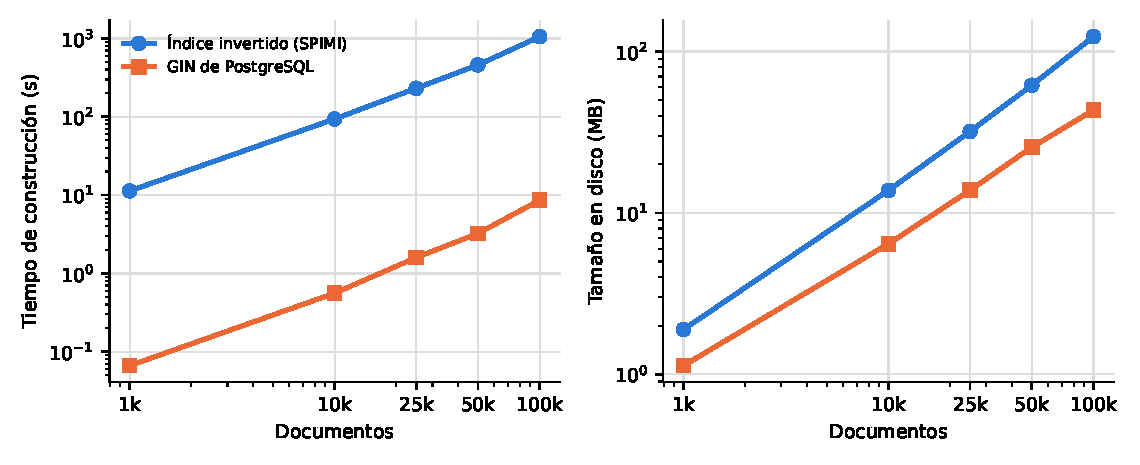
\includegraphics[width=0.95\textwidth]{exp6_construccion}
\caption{Tiempo de construcción y tamaño en disco al crecer el corpus (escala log-log). El índice invertido crece linealmente en tamaño; el GIN crece más lento porque comprime mejor las listas largas.}
\end{figure}

El nuestro crece linealmente: unos 10,5\,ms y 1,2\,KB por documento con 100\,000
documentos. El GIN cuesta 0,09\,ms y 0,4\,KB por documento, y su tamaño crece más lento
que el corpus (de 1,1 a 0,4\,KB por documento) porque las listas largas se comprimen
mejor. La diferencia de tamaño es de diseño: nuestros postings son
registros fijos de 16 bytes sin comprimir que guardan además $tf$ y $|d|$ (los necesita el
ranking sin tocar la tabla), el vocabulario usa claves \code{CHAR(24)} de ancho fijo y hay
un archivo de normas; el GIN comprime las listas (deltas codificados en bytes variables) y
no guarda frecuencias. La diferencia de tiempo (unas 120 veces) viene de que el vocabulario se
arma insertando término por término en el B+ del Proyecto~1 desde Python (468\,239
escrituras de bloque para 100\,000 documentos), mientras que PostgreSQL ordena en memoria y
construye el árbol de abajo hacia arriba en C.

\paragraph{Consultas.}

\begin{table}[H]
\centering\small
\begin{tabular}{rlrrrrrrr}
\toprule
 & & \multicolumn{2}{c}{Índice invertido} & \multicolumn{2}{c}{GIN} & \multicolumn{2}{c}{Full Text Scan} & \\
Términos & Operación & ms & bloques & ms & bloques & ms & bloques & coinciden \\
\midrule
1 & AND (un término) & 273,7 & 4\,155 & 60,3 & 11\,905 & 262\,794 & 25\,000 & 4\,133 \\
1 & Top-10 & 20,5 & 45 & 42,3 & 5\,257 & 283\,671 & 25\,000 & 2\,142 \\
3 & AND & 23,0 & 87 & 0,3 & 40 & 280\,511 & 25\,000 & 20 \\
3 & AND-NOT & 53,0 & 268 & 3,5 & 197 & 265\,128 & 25\,000 & 191 \\
3 & OR & 80,2 & 1\,728 & 14,7 & 1\,388 & 253\,852 & 25\,000 & 1\,682 \\
3 & Top-10 & 29,9 & 72 & 146,0 & 14\,871 & 304\,178 & 25\,000 & 5\,723 \\
5 & AND & 39,8 & 105 & 1,6 & 41 & 261\,475 & 25\,000 & 1 \\
5 & AND-NOT & 44,3 & 122 & 1,9 & 50 & 258\,904 & 25\,000 & 11 \\
5 & OR & 55,0 & 1\,022 & 2,8 & 829 & 253\,416 & 25\,000 & 969 \\
5 & Top-10 & 47,7 & 102 & 389,2 & 67\,941 & 252\,532 & 25\,000 & 9\,727 \\
\bottomrule
\end{tabular}
\caption{Experimento 6b (\code{exp6\_consultas.csv}), $N=100\,000$: latencia y bloques por consulta. ``Coinciden'' es el promedio de documentos que cumplen el \code{MATCH} con el índice. Bloques de 4\,KB en nuestro motor y de 8\,KB en PostgreSQL.}
\end{table}

\begin{figure}[H]
\centering
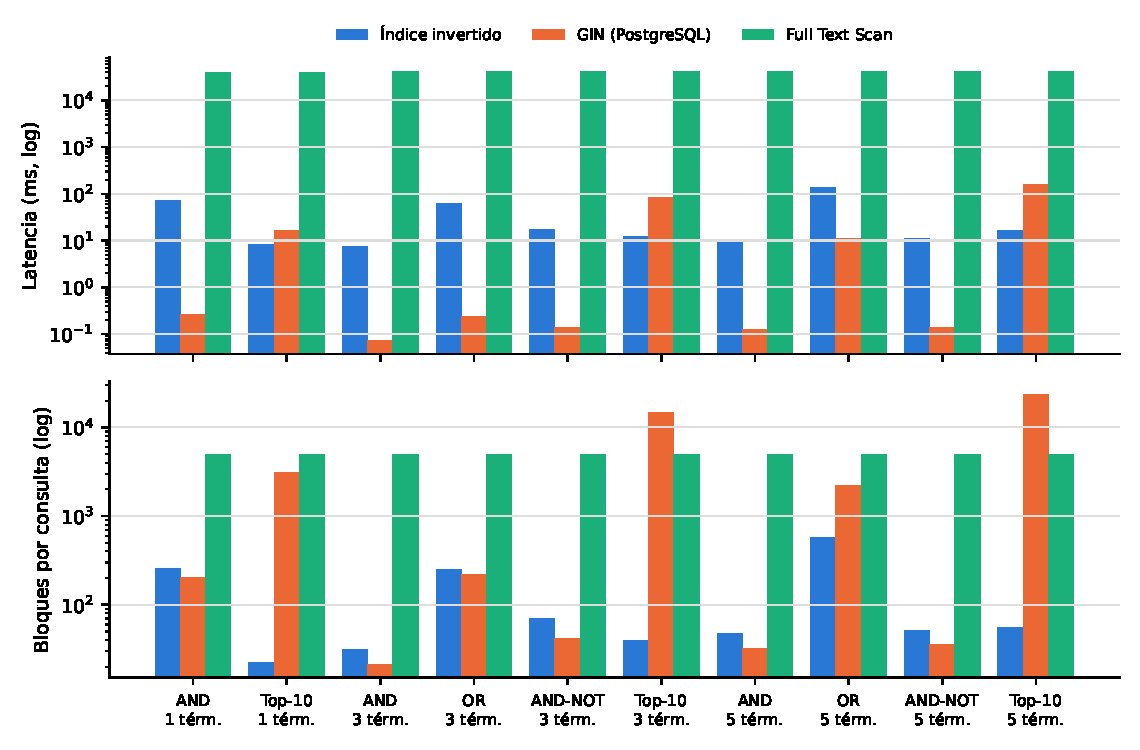
\includegraphics[width=0.95\textwidth]{exp6_consultas}
\caption{Latencia y bloques por consulta (escala logarítmica) de las tres rutas.}
\end{figure}

\paragraph{Análisis.} El Full Text Scan cuesta lo mismo para cualquier consulta: lee las
25\,000 páginas de la tabla y vuelve a preprocesar los 100\,000 documentos (tokenizar, quitar
stopwords, aplicar el stemmer y calcular normas), de 253 a 304 segundos. El índice resuelve las
mismas consultas entre 960 y 13\,800 veces más rápido y con 6 a 560 veces menos bloques. La
parte que lee el índice en sí es pequeña (de 22 a 111 bloques: la altura del B+ más las
páginas de las listas de la consulta); el resto son las filas del resultado traídas de la
tabla, una por documento, porque el \code{SELECT} pide columnas de la tabla. Por eso en
las consultas booleanas los bloques crecen con el número de documentos que cumplen (un
\code{AND} de un solo término trae 4\,133 filas) y, salvo en ese caso, quedan cerca de los
del GIN, que también debe visitar el heap por cada fila.

En las consultas de ranking Top-10 el índice gana a GIN en bloques (de 45 a 102 frente a
5\,257 a 67\,941) y en tiempo (de 20 a 48\,ms frente a 42 a 389\,ms). El score sale entero de
los postings ($tf$ y $|d|$) y de las normas, sin tocar la tabla, así que solo se leen las
10 filas del resultado. \code{ts\_rank} de PostgreSQL, en cambio, necesita el
\code{tsvector} de cada documento que cumple, que vive en el heap: su costo crece con los
5\,723 o 9\,727 documentos que coinciden y no con $k$. Guardar $tf$ y $|d|$ en cada posting
cuesta casi el triple de espacio que el GIN (123,6 frente a 43,4\,MB), y esta es la consulta
donde se recupera.

En las consultas booleanas el GIN es mucho más rápido (de 0,3 a 60\,ms frente a 23 a 274\,ms)
con un número parecido de bloques. Esa diferencia no es de I/O sino de implementación: C
contra Python, y el buffer pool de PostgreSQL contra nuestro motor sin caché, donde cada
acceso cuenta como lectura a propósito para que el \code{DiskCounter} mida la estructura y
no la caché.

Los resultados coinciden: para cada consulta el índice y el Full Text Scan devolvieron
exactamente los mismos documentos (el script lo verifica), y con GIN el número de
documentos difiere en menos de 1\,\% en casi todas las celdas (5\,\% en el Top-10 de un
término), por las pequeñas diferencias entre sus listas de
stopwords y diccionarios y los nuestros.

\section{Módulo vectorial: IVF en disco y planificador híbrido}
\label{sec:vectorial}

% ---------------------------------------------------------------------------
% ROL 3: primera versión redactada por el Rol 4 a partir del README y de
% benchmarks/results/exp8_*.csv para que el informe compile completo. Ajusta lo
% que haga falta (sobre todo el análisis del 8b y los diagramas).
% ---------------------------------------------------------------------------

\subsection{El tipo \code{VECTOR(D)} y la búsqueda exacta}

Un \code{VECTOR(D)} son $D$ \code{float32} contiguos ($4D$ bytes), así que sigue siendo
un tipo de ancho fijo y toda la maquinaria de páginas, bitmap y RID del Proyecto 1 se
aplica sin cambios. Las distancias soportadas son L2 (\code{<->}) y coseno
$1-\cos\theta$ (\code{<=>}). La línea base es el k-NN lineal
(\code{backend/vector/knn.py}): recorre la tabla por lotes, calcula las distancias con
\code{numpy} y mantiene los $k$ mejores en un Max-Heap de tamaño $k$, de modo que un
candidato nuevo se compara con la raíz en $O(1)$ y entra en $O(\log k)$. Es la verdad
de campo del Experimento 8 y la ruta \code{KnnSeqScan} del planificador.

\subsection{Diseño en disco del IVF}

El espacio se parte en $C=\lfloor\sqrt{N}\rfloor$ celdas de Voronoi con K-Means++
(esférico cuando la métrica es coseno). Dos archivos paginados:

\begin{table}[H]
\centering\small
\begin{tabularx}{\textwidth}{llY}
\toprule
Archivo & Registro & Metadatos \\
\midrule
\code{<t>\_\_<idx>.ivf.dir} & $\langle$centroide \code{VECTOR(D)}, cluster\_id, head, tail, count$\rangle$ & \code{user\_a} = métrica, \code{user\_b} = $C$ \\
\code{<t>\_\_<idx>.ivf.lst} & $\langle$pk, page, slot, area, vec$\rangle$, una cadena de páginas por celda & \code{user\_a} = $N$ \\
\bottomrule
\end{tabularx}
\end{table}

Las listas son densas y una página se decodifica de una vez con
\code{numpy.frombuffer}. Se guarda la clave primaria junto al RID porque en este motor
los RID no son estables (move-the-last del Heap, inserción ordenada y
\code{reorganize()} del Sequential): al leer un candidato se verifica la PK y, si el
RID quedó obsoleto, la fila se recupera por clave (\code{plan.stale\_rids}). Los
centroides se leen una vez al abrir el índice y quedan en RAM, como hacen los motores
reales con el cuantizador.

\subsection{Gramática y planificador híbrido}

\begin{lstlisting}
CREATE INDEX idx_vec ON multimedia (embedding) USING IVF WITH (lists = 100, metric = 'COSINE');
SET ivf.probes = 5;
SELECT id, categoria, precio, embedding <=> '[0.12, -0.34, ...]' AS d
FROM multimedia WHERE categoria = 'footwear' AND precio <= 250.0
ORDER BY d ASC LIMIT 5;
\end{lstlisting}

\begin{table}[H]
\centering\small
\begin{tabularx}{\textwidth}{lYY}
\toprule
Situación & Ruta & Qué hace \\
\midrule
sin \code{WHERE}, sin IVF & \code{KnnSeqScan} & k-NN exacto con Max-Heap \\
sin \code{WHERE}, con IVF & \code{IVFScan} & escanea las \code{ivf.probes} celdas más cercanas \\
\code{WHERE} indexable, sin IVF & \code{PreFilter} & B+/Hash entrega candidatos $\to$ k-NN exacto \\
\code{WHERE} no indexable, con IVF & \code{PostFilter} & candidatos IVF en orden $\to$ filtro; amplía el sondeo si no alcanza \\
\code{WHERE} indexable y con IVF & \code{PreFilter} / \code{PostFilter} & decide \code{hybrid.choose\_strategy} con un conteo real del índice \\
\bottomrule
\end{tabularx}
\end{table}

La decisión minimiza bloques leídos: el planificador paga unas pocas páginas del
índice relacional para contar (con tope) cuántas filas cumplen el filtro, estima el
costo de PRE (una lectura de tabla por fila que pasa) y de POST (páginas de las
listas sondeadas más una lectura de tabla por candidato revisado) y, ante empate,
elige PRE porque su resultado es exacto. Cada consulta reporta en \code{plan.io} las
lecturas del índice y de la tabla por separado, que el cliente web dibuja.

\subsection{Experimento 8: eficiencia vs. calidad en ANN}

Datos sintéticos con estructura de clusters ($N=20\,000$, $D=128$, mezcla de 64
gaussianas), 100 consultas, $k=10$, $C=141$ celdas. La verdad de campo es el k-NN
exacto.

\begin{table}[H]
\centering\small
\begin{tabular}{lrrrrr}
\toprule
Método & probes & Recall@10 & ms & bloques & índice / tabla \\
\midrule
k-NN exacto & --- & 1,000 & 210,2 & 2858 & 0 / 2858 \\
IVF & 1 & 0,731 & 7,2 & 38,9 & 28,9 / 10 \\
IVF & 2 & 0,940 & 7,8 & 61,1 & 51,1 / 10 \\
IVF & 5 & 1,000 & 9,6 & 129,8 & 119,8 / 10 \\
IVF & 10 & 1,000 & 12,8 & 252,1 & 242,1 / 10 \\
IVF & 20 & 1,000 & 18,7 & 472,1 & 462,1 / 10 \\
IVF & 50 & 1,000 & 36,4 & 1114,5 & 1104,5 / 10 \\
\bottomrule
\end{tabular}
\caption{Experimento 8a (\code{exp8\_ann.csv}): Recall@10, latencia media y bloques leídos por consulta al variar \code{ivf.probes}.}
\end{table}

\begin{figure}[H]
\centering
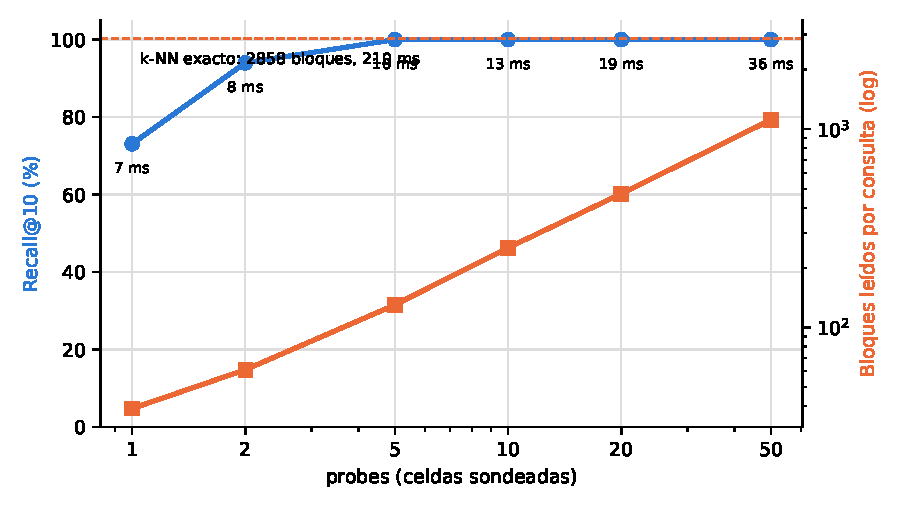
\includegraphics[width=0.78\textwidth]{exp8_recall}
\caption{Curva de compromiso del IVF: el recall crece con \code{probes} mientras los bloques leídos crecen linealmente; con 5 celdas se alcanza recall 1 leyendo 22 veces menos bloques que el escaneo completo.}
\end{figure}

Con una sola celda el IVF ya recupera el 73\,\% de los vecinos verdaderos leyendo
39 bloques frente a los 2858 del escaneo (73 veces menos); con 5 celdas el recall es
1,0 y el costo sigue 22 veces por debajo. A partir de ahí sondear más celdas solo
suma I/O: la curva es la ``rodilla'' clásica del Recall vs.\ costo y justifica el
valor por defecto \code{ivf.probes = 5}. Las 10 lecturas de tabla son constantes
(una página por cada uno de los $k$ resultados), así que todo el costo variable es
del índice.

\begin{table}[H]
\centering\small
\begin{tabular}{rllrrrr}
\toprule
Selectividad & Estrategia & Recall@10 & ms & bloques & índice / tabla & ampliaciones \\
\midrule
0,1\,\% & PRE & 1,00 & 5,0 & 23 & 2 / 21 & 0 \\
0,1\,\% & POST & 0,95 & 3410,4 & 14126,6 & 2407 / 11719 & 3,6 \\
1\,\% & PRE & 1,00 & 8,1 & 204 & 3 / 201 & 0 \\
1\,\% & POST & 0,88 & 281,9 & 1332,8 & 284 / 1048 & 0,65 \\
5\,\% & PRE & 1,00 & 35,3 & 1009 & 8 / 1001 & 0 \\
5\,\% & POST & 1,00 & 83,2 & 333,1 & 126 / 207 & 0 \\
25\,\% & PRE & 1,00 & 126,0 & 5032 & 31 / 5001 & 0 \\
25\,\% & POST & 1,00 & 17,8 & 165,4 & 126 / 39 & 0 \\
100\,\% & PRE & 1,00 & 457,1 & 20124 & 124 / 20000 & 0 \\
100\,\% & POST & 1,00 & 9,9 & 136,3 & 126 / 10 & 0 \\
\bottomrule
\end{tabular}
\caption{Experimento 8b (\code{exp8\_hibrido.csv}): pre- vs.\ post-filtrado con B+ sobre \code{precio} e IVF con 5 probes, forzando la estrategia con \code{SET hybrid.strategy}.}
\end{table}

\begin{figure}[H]
\centering
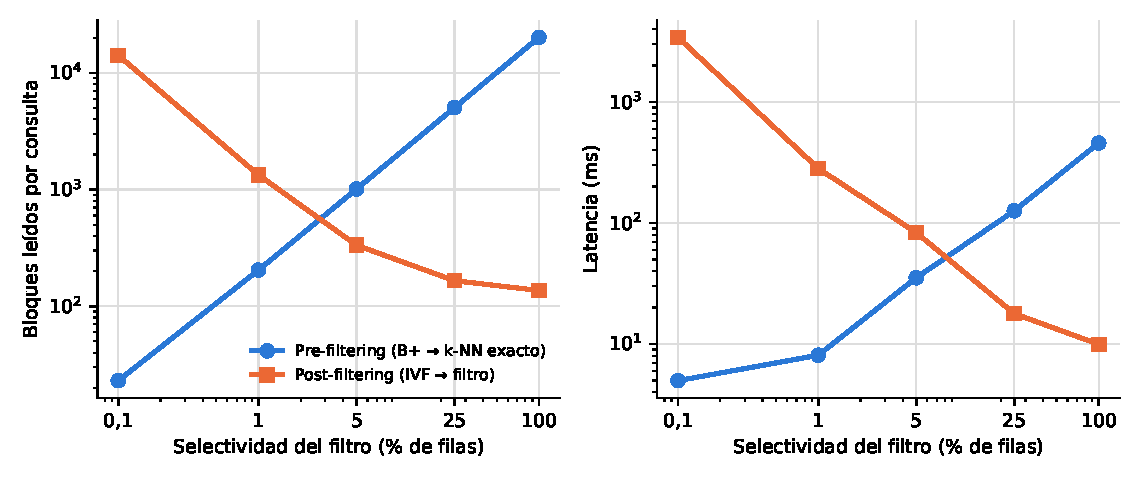
\includegraphics[width=0.95\textwidth]{exp8_hibrido}
\caption{Costo de PRE y POST según la selectividad del filtro. Las curvas se cruzan entre el 1\,\% y el 5\,\%: ahí cambia la decisión del planificador.}
\end{figure}

El cruce está entre 1\,\% y 5\,\% de selectividad. Con filtros muy selectivos el
post-filtrado descarta casi todos los candidatos del IVF y debe ampliar el sondeo
(3,6 veces en promedio al 0,1\,\%), leyendo 600 veces más bloques que el pre-filtrado
y aun así con recall menor que 1; con filtros poco selectivos el pre-filtrado degenera
en un escaneo de la tabla (20\,124 bloques al 100\,\%) mientras el IVF resuelve la
consulta con 136. El estimador del planificador reproduce esta frontera con el conteo
real del índice relacional, que es lo que el Experimento 8b calibra.

\section{Módulo multimedia y aplicación de IA}
\label{sec:multimedia}

Esta sección cubre el enunciado 5.3.1 (representación clásica frente a embeddings
densos), la aplicación vertical de la sección 5.5 (opción A: RAG) y el Experimento 7.
La regla de diseño fue no inventar almacenamiento nuevo: cada representación termina
en una tabla \code{HEAP} con una columna \code{VECTOR(D)} o en el índice invertido de
la sección~\ref{sec:textual}, y cada consulta pasa por el planificador de la
sección~\ref{sec:vectorial} o por los postings en disco, con el \code{DiskCounter}
contando.

\subsection{Dos representaciones de una imagen}

\paragraph{Paradigma clásico: Bag of Visual Words.}
SIFT (OpenCV) produce para cada imagen unos cientos de descriptores locales de 128
dimensiones, invariantes a escala y rotación. Un \emph{codebook} de $K$ palabras
visuales se entrena con K-Means (variante \emph{mini-batch} de scikit-learn) sobre una
muestra estratificada de descriptores de 1\,500 imágenes; después cada descriptor de
cada imagen se cuantiza a su centroide más cercano y la imagen queda representada por
la bolsa \code{["vw0012", "vw0012", "vw0377", \ldots]}. Esa lista entra al mismo SPIMI
que los documentos de texto: \code{build\_index(\ldots, tokenize=identidad)} salta
stopwords y stemming, porque una palabra visual no tiene morfología. La consulta es
TF-IDF logarítmico con similitud de coseno,

\[
  w_{t,d} = (1+\log_{10} tf_{t,d})\cdot\log_{10}\frac{N}{df_t},\qquad
  \mathrm{score}(q,d)=\frac{\sum_{t\in q} w_{t,q}\,w_{t,d}}{\lVert d\rVert_2\,\lVert q\rVert_2},
\]

donde la norma $\lVert d\rVert_2$ se precalcula al construir el índice y se guarda en
disco en \code{<base>.norms.dat}, un archivo paginado de registros
$\langle$page, slot, norma$\rangle$ (16 bytes). Las normas se leen una vez al abrir el
índice y quedan en RAM, con el mismo criterio que los centroides del IVF: son $N$
flotantes y releerlas en cada consulta solo añadiría ruido a la comparación. El
codebook se persiste como la tabla \code{codebook\_bovw(id INT, centro VECTOR(128))},
así que la aplicación lo recupera con un \code{scan} y no hay serializador externo.

\paragraph{Paradigma moderno: embeddings densos.}
ResNet-18 preentrenada en ImageNet, sin la capa de clasificación: el vector de 512
dimensiones del \emph{average pooling}, normalizado a norma 1. Va en la columna
\code{emb VECTOR(512)} de la tabla \code{imagenes(id, categoria CHAR(20), archivo
CHAR(64), emb)} y se indexa con \code{CREATE INDEX idx\_emb ON imagenes (emb) USING IVF
WITH (metric = 'COSINE')}. La consulta es SQL ordinario del módulo vectorial:

\begin{lstlisting}
SELECT id, categoria, archivo, emb <=> '[...]' AS dist
FROM imagenes ORDER BY dist ASC LIMIT 10;      -- IVFScan (o KnnSeqScan con <->)
\end{lstlisting}

\begin{figure}[H]
\centering
\begin{tikzpicture}[
  node distance=3mm and 5mm,
  caja/.style={draw, rounded corners=1pt, align=center, font=\footnotesize, inner sep=3pt, minimum height=7mm},
  flecha/.style={-{Latex[length=1.8mm]}, thick},
]
\node[caja] (img) {imagen};
\node[caja, above right=2mm and 8mm of img, fill=blue!6] (sift) {SIFT\\ $n\times128$};
\node[caja, right=of sift, fill=blue!6] (cb) {codebook\\ K-Means ($K$)\\ tabla \code{codebook\_bovw}};
\node[caja, right=of cb, fill=blue!6] (bag) {bolsa de palabras\\ \code{vw0012 vw0377 \ldots}};
\node[caja, right=of bag, fill=green!6] (inv) {índice invertido\\ vocab B+ + postings\\ + \code{norms.dat}};
\node[caja, below right=2mm and 8mm of img, fill=orange!8] (cnn) {ResNet-18\\ avgpool 512-D};
\node[caja, right=of cnn, fill=orange!8] (tab) {\code{imagenes.emb}\\ \code{VECTOR(512)}};
\node[caja, right=of tab, fill=green!6] (ivf) {IVF COSINE\\ \code{.ivf.dir} + \code{.ivf.lst}};
\node[caja, right=of ivf] (q2) {\code{ORDER BY emb <=> q}\\ \code{LIMIT k}};
\node[caja, right=of inv] (q1) {TF-IDF coseno\\ top-$k$ (heap)};
\draw[flecha] (img) -- (sift); \draw[flecha] (sift) -- (cb); \draw[flecha] (cb) -- (bag); \draw[flecha] (bag) -- (inv); \draw[flecha] (inv) -- (q1);
\draw[flecha] (img) -- (cnn); \draw[flecha] (cnn) -- (tab); \draw[flecha] (tab) -- (ivf); \draw[flecha] (ivf) -- (q2);
\end{tikzpicture}
\caption{Los dos caminos de una imagen. Arriba el clásico (SIFT $\to$ palabras visuales $\to$ índice invertido), abajo el moderno (CNN $\to$ \code{VECTOR} $\to$ IVF). Los dos terminan en archivos paginados del motor.}
\end{figure}

\subsection{Texto: SBERT sobre el mismo motor}

Para el corpus del RAG el embedding es SBERT multilingüe
(\code{paraphrase-multilingual-MiniLM-L12-v2}, 384 dimensiones), calculado sobre
``título. texto'' para que el título pese en la representación. La tabla
\code{documentos(id, lang CHAR(2), titulo CHAR(80), texto CHAR(1000), emb VECTOR(384))}
ocupa un registro por página de 4 KB (2\,622 bytes), lo que hace muy visible la
diferencia entre leer la tabla y leer un índice. Sobre ella conviven el IVF
(\code{idx\_emb}, métrica coseno) y el índice invertido SPIMI construido con el
pipeline léxico del Rol 2, sobre cuyos postings corren tanto BM25 como el TF-IDF
coseno de esta sección. Todos los índices textuales viven en \code{data/text/} porque
el catálogo descubre los índices relacionales por el nombre del archivo y el
vocabulario, que es un B+ de términos, no debe aparecer como un índice de la tabla.

\subsection{Aplicación de IA: RAG sobre Wikipedia}

\paragraph{Corpus.} 15\,000 artículos de Wikipedia (7\,500 en español y 7\,500 en
inglés, dump 20231101 vía la API de filas de Hugging Face), con el inicio de cada
artículo recortado a 1\,000 bytes. El descargador (\code{backend/rag/download.py})
reanuda desde donde quedó el CSV y respeta el límite de tasa del servidor
(HTTP 429) con espera exponencial, porque la API corta alrededor de las 5\,000 filas
seguidas.

\paragraph{Flujo.} Ante una pregunta en lenguaje natural el servicio
(\code{backend/rag/pipeline.py}) ejecuta las dos recuperaciones y las devuelve lado a
lado:

\begin{enumerate}[nosep]
  \item \textbf{léxica}: términos de la consulta $\to$ vocabulario B+ $\to$ solo las
        listas de posteo de esos términos $\to$ TF-IDF coseno (o BM25) $\to$ top-$k$;
  \item \textbf{semántica}: SBERT(pregunta) $\to$ \code{SELECT \ldots ORDER BY emb <=>
        '[\ldots]' LIMIT k} $\to$ el planificador elige \code{IVFScan} (con
        \code{SET ivf.probes}) o \code{KnnSeqScan};
  \item \textbf{prompt}: los $k$ fragmentos numerados (semánticos, léxicos o la fusión
        por rango de ambas listas) más la pregunta, con la instrucción de responder en
        el idioma de la pregunta y citar \code{[n]};
  \item \textbf{generación}: el cliente \code{backend/rag/llm.py} es independiente del
        proveedor (SDK de Anthropic, cualquier API compatible con
        \code{/chat/completions} ---Gemini, Groq, OpenAI, Ollama--- o un modelo local
        con \code{transformers}); sin clave cae a una respuesta \emph{extractiva} que
        mantiene demostrable el resto del pipeline.
\end{enumerate}

El cliente web muestra la respuesta con las citas enlazadas a las fuentes, los
fragmentos de cada ruta con su score y, para cada ruta, la ruta de acceso, la latencia
y los bloques leídos del índice y de la tabla. Es el mismo desglose que exige el
planificador híbrido, aplicado a una aplicación completa.

\paragraph{Interfaz multimedia.} La segunda vista permite subir una foto o elegir una
imagen indexada como consulta y devuelve el top-$k$ de los dos paradigmas con
miniaturas, el tiempo de extracción (SIFT + cuantización frente al paso por la CNN),
la latencia, el I/O y ---cuando la consulta es una imagen del dataset--- la
Precision@$k$ por categoría, marcando en verde los aciertos.

\subsection{Experimento 7: paradigma clásico vs. embeddings densos}

\paragraph{Metodología.} Caltech-101 completo sin la carpeta de fondo (8\,677
imágenes, 101 categorías). Consultas: 5 imágenes al azar de cada una de las 30
categorías más pobladas (150 consultas); una imagen recuperada es relevante si tiene la
categoría de la consulta y la propia consulta se excluye del ranking. Métodos: BoVW con
$K\in\{128,256,512\}$ sobre el índice invertido con TF-IDF coseno; ResNet-18 con k-NN
exacto (\code{KnnSeqScan}, verdad de campo del IVF) y con IVF y
\code{probes}$\in\{1,5,20\}$. Se mide Precision@5, Precision@10, el tiempo de
extracción por imagen (SIFT + cuantización frente al \emph{forward} por lotes de la
CNN), la latencia de consulta y los bloques leídos del índice y de la tabla. El bloque
7b repite la comparación en texto con una búsqueda de ítem conocido sobre Wikipedia
(consulta = título del artículo): TF-IDF coseno y BM25 frente a SBERT exacto e IVF.

\begin{table}[H]
\centering\footnotesize\setlength{\tabcolsep}{4pt}
\begin{tabular}{lrrrrrrr}
\toprule
Método & P@5 (\%) & P@10 (\%) & extracción (ms/img) & consulta (ms) & bloques & índice / tabla & índice (KB) \\
\midrule
BoVW, $K=128$ & 10,8 & 8,8 & 11,9 & 971,1 & 2\,703 & 2\,692 / 11 & 13\,132 \\
BoVW, $K=256$ & 14,4 & 12,5 & 11,9 & 1\,057,5 & 3\,085 & 3\,074 / 11 & 19\,292 \\
BoVW, $K=512$ & 19,3 & 16,5 & 11,6 & 964,8 & 2\,928 & 2\,917 / 11 & 25\,240 \\
ResNet-18, k-NN exacto & 87,1 & 85,9 & 17,2 & 358,6 & 8\,677 & 0 / 8\,677 & 0 \\
ResNet-18, IVF probes=1 & 86,3 & 85,7 & 17,2 & 6,0 & 117 & 106 / 11 & 35\,088 \\
ResNet-18, IVF probes=5 & 87,3 & 86,5 & 17,2 & 13,4 & 509 & 498 / 11 & 35\,088 \\
ResNet-18, IVF probes=20 & 87,2 & 86,0 & 17,2 & 39,2 & 1\,880 & 1\,869 / 11 & 35\,088 \\
\bottomrule
\end{tabular}
\caption{Experimento 7a (\code{exp7\_imagenes.csv}): Caltech-101, 8677 imágenes de 101 categorías, 150 consultas. Precisión = fracción del top-$k$ con la misma categoría que la consulta (sin contar la propia imagen).}
\label{tab:exp7a}
\end{table}

\begin{table}[H]
\centering\footnotesize\setlength{\tabcolsep}{4pt}
\begin{tabular}{lrrrrrrr}
\toprule
Método & hit@1 (\%) & hit@10 (\%) & MRR@10 & consulta$\to$vector (ms) & búsqueda (ms) & bloques & índice / tabla \\
\midrule
TF-IDF + coseno & 77,3 & 96,3 & 0,844 & 0,1 & 1,6 & 16 & 9 / 7 \\
BM25 & 84,7 & 96,7 & 0,892 & 0,1 & 1,5 & 16 & 9 / 7 \\
SBERT, k-NN exacto & 77,3 & 89,3 & 0,820 & 11,4 & 158,5 & 4\,000 & 0 / 4\,000 \\
SBERT, IVF probes=1 & 48,3 & 54,3 & 0,507 & 10,3 & 5,8 & 48 & 38 / 10 \\
SBERT, IVF probes=5 & 68,3 & 77,0 & 0,720 & 10,2 & 9,0 & 191 & 181 / 10 \\
SBERT, IVF probes=20 & 75,0 & 86,7 & 0,795 & 10,7 & 20,8 & 674 & 664 / 10 \\
\bottomrule
\end{tabular}
\caption{Experimento 7b (\code{exp7\_texto.csv}): Wikipedia es/en, 4000 artículos, 300 consultas de ítem conocido (la consulta es el título; acierto = recuperar ese artículo).}
\label{tab:exp7b}
\end{table}


\begin{figure}[H]
\centering
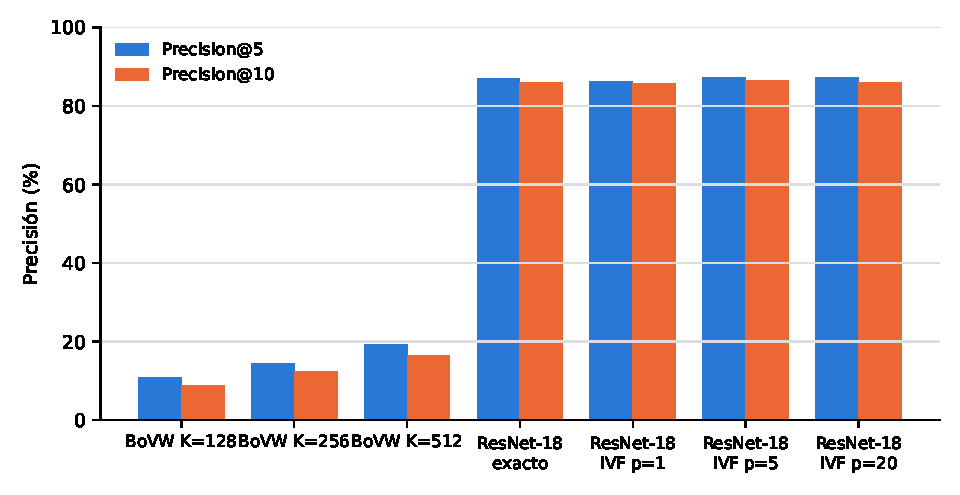
\includegraphics[width=0.85\textwidth]{exp7_precision}
\caption{Precision@5 y @10 por método en Caltech-101.}
\end{figure}

\begin{figure}[H]
\centering
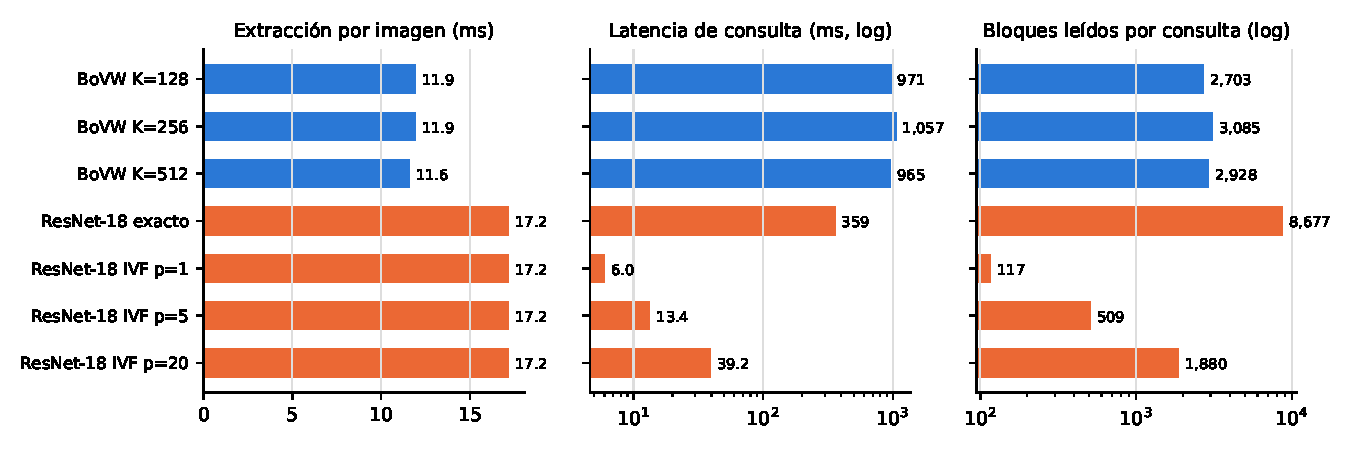
\includegraphics[width=\textwidth]{exp7_costos}
\caption{Costo de cada método: extracción por imagen, latencia de consulta y bloques leídos (escala logarítmica donde la diferencia lo exige).}
\end{figure}

%%ANALISIS7A%%

\begin{figure}[H]
\centering
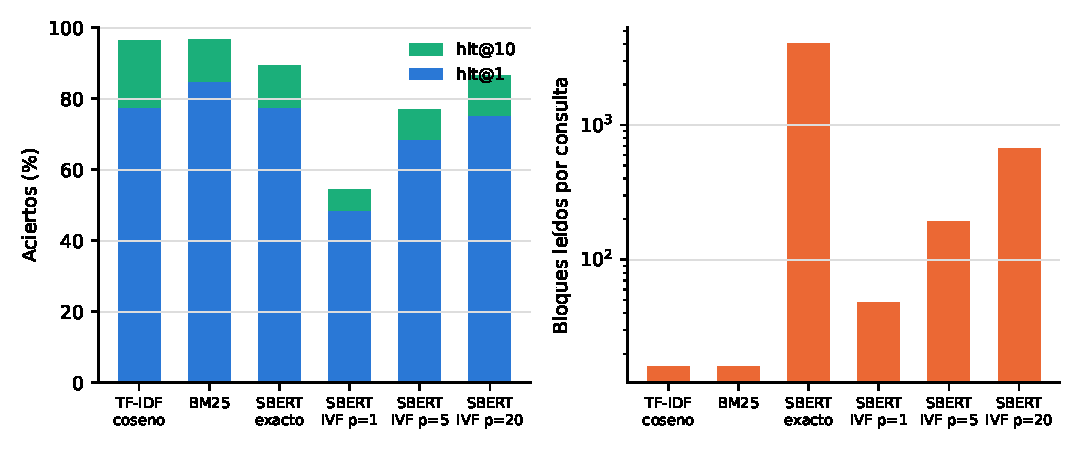
\includegraphics[width=0.9\textwidth]{exp7_texto}
\caption{Experimento 7b: aciertos de ítem conocido y bloques leídos por consulta, léxico frente a SBERT.}
\end{figure}

%%ANALISIS7B%%

\section{Conclusiones}

\begin{itemize}
  \item \textbf{La misma página sirve para todo.} R-Tree, vocabulario, postings,
        normas, directorio y listas del IVF reutilizan la cabecera de 32 bytes y el
        \code{Pager} del Proyecto 1. Eso hizo que el desglose de I/O por consulta
        ---bloques del índice frente a bloques de la tabla--- fuera comparable entre
        los cuatro módulos y entre los dos paradigmas multimedia sin instrumentación
        adicional.
  \item \textbf{Cada índice gana en su régimen y pierde fuera de él.} El R-Tree deja de
        servir cuando las cajas se solapan (dimensión alta); el IVF cambia recall por
        bloques y la rodilla aparece con pocas celdas; el pre-filtrado relacional gana
        con filtros selectivos y el post-filtrado con filtros laxos. El planificador
        híbrido existe para elegir el régimen con datos del propio índice.
  \item \textbf{Las representaciones aprendidas dominan a las cuantizadas en calidad,
        no necesariamente en costo.} En el Experimento 7 el embedding denso supera
        ampliamente a BoVW en Precision@$k$, mientras que la extracción SIFT es más
        barata y el índice invertido lee pocas páginas por consulta. En el texto, la
        recuperación léxica sigue siendo la mejor para consultas de ítem conocido y la
        semántica la complementa en consultas parafraseadas; por eso el RAG muestra
        ambas rutas lado a lado y permite fusionarlas.
  \item \textbf{La aplicación de IA no necesitó estructuras fuera del motor.} Corpus,
        embeddings, codebook e imágenes indexadas son tablas e índices consultables con
        el mismo SQL del cliente web, y el modelo de lenguaje solo consume los
        fragmentos que el planificador recuperó.
\end{itemize}


\end{document}
